\documentclass[11pt,a4paper]{article}

\usepackage[utf8]{inputenc}
\usepackage[T1]{fontenc}
\usepackage{lmodern}
\usepackage[margin=2.5cm]{geometry}
\usepackage{amsmath,amssymb}
\usepackage{graphicx}
\usepackage{booktabs}
\usepackage{adjustbox}
\usepackage{caption}
\usepackage{enumitem}
\usepackage[authoryear,round]{natbib}
\usepackage[hidelinks]{hyperref}
\usepackage{microtype}
\captionsetup{font=small,labelfont=bf}
\setlength{\emergencystretch}{3em}

\newcommand{\NRMSE}{\mathrm{NRMSE}}
\newcommand{\SSC}{SSC}
\newcommand{\Real}{\mathbb{R}}
\newcommand{\placeholder}[1]{\textbf{[#1]}}
\newcommand{\nRepTwoDone}{8}
\newcommand{\nAdaTwoDone}{5}
\newcommand{\nSemiDone}{0}


\title{Finding the edges is not enough: an evaluation of edge-function recovery in sparse additive-noise DAG learners}
\author{[Author list to be completed by the authors]}
\date{Preprint, draft of \today}

\begin{document}
\maketitle

\begin{abstract}
Nonlinear additive-noise DAG learners are valued because every edge is an inspectable function, yet benchmarks score only whether the edges are found. We evaluate the recovered edge functions against ground truth in simulation, using an edge-function error (NRMSE), an interventional-effect error and calibration measures. A screened, group-lasso spline learner (SPADE-scaled) recovers structure almost perfectly on internally standardised data (AUROC 0.997--0.999 for $d=100$ to $500$), but its edge curves keep a median of about 44\% of the true amplitude in the main cell and 14--46\% across cells (edge-function NRMSE 0.61--0.80) and the interventional-effect curves derived from them are wrong even for direct parents (NRMSE 0.58--0.76). On fresh seeds (75 datasets, eight cells, $d=100$ and $200$) we compare three repairs: an unpenalised refit on the selected support (NRMSE 0.20--0.47), the standard adaptive group lasso (0.24--0.52, structure unchanged, AUROC 0.998), and BASIL-W, a Bayesian model-averaged estimator warm-started from the learner's causal order (0.15--0.29, lower than SPADE-scaled in all 75 datasets). The adaptive group lasso closes about 85\% of the gap between SPADE-scaled and BASIL-W at no structural cost. BASIL-W is clearly better than the refit only under non-uniform noise, supplies calibrated edge probabilities, but costs 0.006--0.032 AUROC, its 90\% credible bands cover only 74--81\% of the truth, and on the real Sachs data no repair improves structure while the refit and BASIL-W are much less stable than SPADE-scaled because edges flip in and out of the selected set. None of the repair ingredients is new; our contribution is the measurement, the metrics, the pre-registered paired comparison and the negative results.
\end{abstract}

\paragraph{Keywords.} causal discovery; additive noise models; edge functions; group lasso; Bayesian order MCMC; evaluation.

%=====================================================================
\section{Introduction}
\label{sec:intro}

Differentiable learners for nonlinear additive-noise structural equation models (ANMs) are often motivated by interpretability: each edge $c\to e$ is a univariate function $f_{ce}$ that a practitioner can plot, and the shape (saturating, threshold-like, non-monotone) is meant to carry information beyond the presence of the edge \citep{agarwal2021,liu2025kan,dang_spade}. Published evaluations of such learners, and of nonlinear DAG learners in general, report structure metrics (SHD, SID, AUROC) \citep{zheng2020,lachapelle2020,rolland2022,montagna2023nogam}. Whether the returned functions are \emph{correct} is rarely scored, although a sparsity-inducing group penalty is known to bias the amplitude of the selected components towards zero \citep{huang2010,belloni2013}.

This paper asks a narrow question in a controlled setting: when a sparse spline additive DAG learner finds the edges, how accurate are the functions it returns, how much does that matter for the interventional effects a user would read off the model, and which fixes work? We answer it by simulation with ground-truth edge functions at $d=100$ to $500$, by a pre-registered paired comparison of repair strategies on fresh seeds, and by a real-data check on the Sachs protein-signalling data where function ground truth does not exist.

\paragraph{Framing.} This is an \emph{evaluation study}. It does not propose a new estimator. One of the estimators we compare (BASIL-W) was developed by us in the course of the project; we report it as one candidate among several and disclose that its ingredients are established (Section~\ref{sec:novelty}).

\paragraph{Contributions.} We claim the following, and nothing beyond it.
\begin{enumerate}[leftmargin=*,itemsep=2pt]
  \item \textbf{A measurement.} A structure-accurate learner (SPADE-scaled, AUROC 0.997--0.999) returns edge functions with a median of 14--46\% of the true amplitude, depending on the cell, and the shortfall persists across four noise families, three sample sizes, a second mechanism family and $d$ up to 500 (Section~\ref{sec:rep}). To our knowledge this has not been quantified against ground truth for additive spline or KAN-type DAG learners; the evidence for ``not done before'' is absence of search hits, not proof.
  \item \textbf{Metrics.} An edge-function NRMSE over true edges (a missed edge counts as an error of 1), a calibration slope, and an interventional (do-effect) NRMSE for direct and indirect pairs propagated through the learned model, together with edge-probability calibration (ECE) and band coverage (Section~\ref{sec:metrics}). The do-effect error follows the established idea of interventional evaluation \citep{gentzel2019}; we do not claim it as new.
  \item \textbf{A paired comparison of repairs} that includes the standard adaptive group lasso \citep{huang2010}, an unpenalised refit, and a Bayesian estimator, with the protocol fixed by git commits before the runs (Section~\ref{sec:protocol}). The main finding is deflationary: the adaptive group lasso removes most of the shrinkage without changing the selected structure.
  \item \textbf{Negative results.} A group-MCP learner with an independence term (SPIRE) loses structure accuracy; the cold-start Bayesian scaling variant (BASIL-S) does not converge at $d\ge100$; full BASIL does not scale; the pre-registered BASIL-W had a numerical instability in interventional effects; BASIL-W lowers AUROC in every dataset; its credible bands under-cover; and on Sachs the repairs are less stable than the unrepaired learner (Sections~\ref{sec:bands}, \ref{sec:sachs}, \ref{sec:neg}).
\end{enumerate}

\paragraph{What is not new.} The unpenalised refit on a selected support is post-lasso least squares \citep{belloni2013}. The adaptive group lasso for spline additive models is due to \citet{huang2010}. The ingredients of BASIL-W (closed-form marginal likelihoods with a $g$-prior, order MCMC, spline-based Bayesian DAGs, model averaging over parent sets) are due to \citet{friedman2003}, \citet{ni2015}, \citet{toth2025} and others. Independence-based criteria combined with adaptive group sparsity appear in a concurrent ICML 2026 paper \citep{yao2026}, which we know only from its abstract. Interventional evaluation is advocated by \citet{gentzel2019}. We found no prior work that combines these in the way BASIL-W does or that defines the edge-function NRMSE, but this rests on a limited search (Section~\ref{sec:related}).

\paragraph{Scope of causal claims.} Everything here assumes an additive-noise model with causal sufficiency. We make no claim about causal validity of any learned graph or function beyond these assumptions; the heteroscedastic cell violates additivity on purpose and the real-data results are weak.

\paragraph{Outline.} Section~\ref{sec:related} reviews related work, Section~\ref{sec:metrics} defines the problem and metrics, Section~\ref{sec:methods} the methods, Section~\ref{sec:protocol} the protocol, Section~\ref{sec:results} the results, Section~\ref{sec:discussion} discusses limitations, and Section~\ref{sec:repro} gives reproducibility details.

%=====================================================================
\section{Related work}
\label{sec:related}

\paragraph{Identifiability and continuous DAG learning.} Nonlinear additive-noise models make the DAG identifiable \citep{hoyer2008,peters2014}. NOTEARS \citep{zheng2018} turned structure search into continuous optimisation with a smooth acyclicity penalty; NOTEARS-MLP \citep{zheng2020}, GraN-DAG \citep{lachapelle2020}, GOLEM \citep{ng2020} and DAGMA \citep{bello2022} extended it to nonparametric models and better-conditioned constraints, and truncated matrix power iteration \citep{zhang2022tmpi} reduces its cost. Order-based methods split the problem: CAM \citep{buhlmann2014} searches orders under additive models and prunes with sparse regression, SCORE \citep{rolland2022}, NoGAM \citep{montagna2023nogam} and DAS \citep{montagna2023das} obtain the order from score matching, and DiffAN does so with diffusion models \citep{sanchez2023}. These works report structure metrics. Evaluation caveats are well documented: varsortability and R$^2$-sortability \citep{reisach2021,reisach2023}, scale sensitivity of NOTEARS \citep{kaiser2021,seng2024}, and internally standardised generators \citep{ormaniec2025}, which we use. \citet{montagna2023assumptions} study robustness of score matching to assumption violations, in the spirit of our heteroscedastic cell.

\paragraph{Additive and spline models, and sparsity bias.} Sparse additive models \citep{ravikumar2009} and the adaptive group lasso for spline additive models \citep{huang2010} select components by group penalties; the latter shows that adaptive weights restore selection consistency by reducing the bias on strong groups. Refitting after selection is classical: least squares after selection has smaller bias than the lasso \citep{belloni2013}, and the adaptive lasso \citep{zou2006} was designed for the same purpose. In DAG learning, an adaptive lasso has been proposed to avoid hard thresholding that deletes small true edges \citep{xu2022}. Neural Granger causality uses first-layer group lasso for selection \citep{tank2022}. A concurrent ICML 2026 paper combines an independence criterion with an adaptive group lasso on first-layer MLP weights to prune constant edges under non-Gaussian, heteroscedastic noise \citep{yao2026}; we read only its abstract, which states a focus on identifiability and structure, not on recovery of edge amplitudes. We found no study that measures how group-lasso shrinkage distorts the amplitude of recovered edge functions in additive DAG learners; accordingly we treat the plain refit and adaptive penalties as baselines.

\paragraph{Interpretable edge functions.} Neural additive models \citep{agarwal2021} and KANs \citep{liu2025kan}, with critiques by \citet{yu2024kan} and \citet{hou2024kan}, promise readable univariate components. Dagma-DCE \citep{waxman2024} replaces weight norms by a derivative-based causal-effect strength. In time series, NAVAR \citep{bussmann2021} is additive, and \citet{kuskova2026} estimate function-valued causal influence from trained NAVAR models and show that equal scalar scores can hide different shapes; in the part we read (abstract only) they do not report an accuracy metric against known functions. Concurvity can make additive components non-identifiable \citep{siems2023}. To our knowledge no benchmark scores recovered edge functions against ground truth in cross-sectional nonlinear causal discovery. Interventional evaluation of causal models has been advocated \citep{gentzel2019}, and recent Bayesian work reports errors of average causal effects \citep{toth2025}; our do-effect error follows this line.

\paragraph{Bayesian structure learning.} Order MCMC \citep{friedman2003} samples node orders and sums over parent sets; its prior bias towards graphs compatible with many orders is analysed by \citet{viinikka2020}. Nonlinear Bayesian structure learners include Gaussian process networks with marginal-likelihood scores \citep{friedman2000}, spline-based Bayesian DAGs with edge and functional selection \citep{ni2015}, DiBS \citep{lorch2021}, BayesDAG \citep{annadani2023} and structural marginalisation with autoregressive orders for Gaussian-process additive models \citep{toth2025}. \citet{wang2025orderings} build confidence sets for causal orderings under additive errors. Our estimator BASIL-W combines a $g$-prior closed-form marginal likelihood on spline features with order MCMC warm-started from a continuous learner. Its ingredients are established and we do not claim the inference idea as new.

\subsection{What is and is not new here}
\label{sec:novelty}
Not new: the refit, the adaptive group lasso, the Bayesian ingredients, interventional evaluation, the idea of independence plus adaptive group sparsity. Possibly new, subject to the limits of our search: the edge-function NRMSE and the study of amplitude shrinkage in spline additive DAG learners against ground truth; the particular combination BASIL-W and its warm start from a continuous learner. The literature check was performed with web search only, mostly at the level of abstracts and snippets, and absence of a hit is weak evidence.

%=====================================================================
\section{Problem and metrics}
\label{sec:metrics}

\paragraph{Model.} Data $x\in\Real^d$ follow an additive-noise SEM $x_e=\sum_{c\in\mathrm{pa}(e)} f_{ce}(x_c)+\varepsilon_e$ with $\varepsilon_e$ independent of $x_{\mathrm{pa}(e)}$ and a DAG $A$. Generation is internally standardised (iSCM, \citealt{ormaniec2025}): each variable is standardised right after it is generated, so that no learner can exploit marginal variance as a causal-order cue \citep{reisach2021}. The true edge function in standardised units is $g^\ast_{ce}(x)=f_{ce}(x)/s_e$, where $s_e$ is the standard deviation of the generated (unstandardised) variable. We always compare centred curves on the observed values of the cause.

\paragraph{Edge-function NRMSE (primary metric).} For a true edge $c\to e$ with estimated curve $\hat g_{ce}$ (zero if the edge is not selected),
\[
\NRMSE_{ce}=\frac{\lVert \hat g_{ce}-g^\ast_{ce}\rVert_2}{\lVert g^\ast_{ce}\rVert_2},
\]
evaluated on the $n$ observed values of $x_c$ after centring both curves. A missed edge has $\hat g=0$ and an error of 1; an estimate with the right shape and half the amplitude has an error of 0.5. The dataset-level value is the mean over its true edges; the dataset is the unit of analysis. We also report the calibration slope $\langle\hat g,g^\ast\rangle/\langle g^\ast,g^\ast\rangle$ (median over edges; 1 is ideal, a slope of 0.44 means 44\% of the true amplitude), and the curve R$^2$.

\paragraph{Do-effect NRMSE.} For a pair $(c,e)$ the interventional curve $\tau_{ce}(v)=\mathbb{E}[x_e\mid \mathrm{do}(x_c=v)]$ is evaluated on a 15-point grid between the 5th and 95th percentile of $x_c$. The truth is obtained by Monte Carlo (1000 draws) from the true SEM. The learned curve is obtained by propagating the intervention through the learned SEM in a topological order of the learned graph (source peeling on edge strength), keeping the observed residuals; 400 rows are used. The error is $\lVert\hat\tau-\tau\rVert/\lVert\tau\rVert$ after centring. Up to 20 \emph{direct} (true parent) and 20 \emph{indirect} (true ancestor, not parent) pairs are drawn per dataset; pairs whose true curve has standard deviation below 0.05 are skipped (about 3.8 of about 40 per dataset, identically for all methods). Indirect pairs test whether errors accumulate along paths.

\paragraph{Structure metrics.} Directed AUROC over all ordered pairs against the true adjacency, AUPRC, and orientation accuracy on the true edges (1 if the score for the true direction exceeds the reversed one, $0.5$ for ties). Edge scores are the standard deviation of the edge's contribution (learners) or posterior edge probabilities (Bayesian estimators).

\paragraph{Calibration.} For the Bayesian estimators: expected calibration error (ECE, 10 bins) of edge probabilities over off-diagonal pairs; pointwise coverage of the 90\% credible band of $g_{ce}$ over true edges and rows, where a missed edge has a band concentrated at zero and therefore usually fails to cover.

%=====================================================================
\section{Methods}
\label{sec:methods}

\subsection{SPADE-scaled (SSC)}
SPADE \citep{dang_spade} represents every edge as a cubic B-spline function on a fixed grid (grid size 8 on $[-3,3]$, 11 coefficients per edge), regresses each variable on spline functions of its candidate parents, and penalises each edge's coefficient group with a group lasso under an acyclicity constraint. The scaled variant used here (SSC) adds two changes that were fixed on an earlier generator: tree-ensemble screening to $K=15$ candidate parents per node, and a penalty $\lambda=0.2/d$ instead of a fixed $\lambda$, because a group penalty summed over $d(d-1)$ candidate edges over-penalises as $d$ grows. It is trained for 400 epochs. The edge score is the standard deviation of the edge's contribution on the data. SSC is the baseline against which all repairs are measured.

\subsection{Refit (SSR)}
The $\lceil 1.5\,d\rceil$ highest-scoring edges of SSC define a support (``top $1.5d$''; the multiplier $k=1.5$ was chosen on three validation datasets at $d=100$, among $k\in\{1,1.5,2\}$ and uses the knowledge that the generating graphs have about $d$ edges). The model is refit from scratch on this mask with $\lambda=0$. This is post-lasso least squares in the sense of \citet{belloni2013}.

\subsection{Adaptive group lasso (SSA)}
A second fit of SSC, on the same screened candidates and the same $\lambda=0.2/d$, with edge-wise weights $w_{ce}=(\lVert\theta_{ce}\rVert+0.01)^{-1}$ computed from the first SSC fit and normalised to mean 1 over the screened edges. This is the adaptive group lasso of \citet{huang2010} with exponent $\gamma=1$ and offset $\epsilon=0.01$. Neither was tuned on any dataset in this paper's main grids. (A sensitivity analysis is in Section~\ref{sec:adaptive2}.)

\subsection{BASIL-W}
BASIL-W (Bayesian spline additive structure learning, warm-started) averages over parent sets and orders. Spline features of each candidate parent are whitened, and for a node $i$ with parent set $S$ ($|S|\le k_{\max}=3$) the marginal likelihood is available in closed form under a Zellner $g$-prior with $g=n$ and a per-parent log-odds prior $\log(\pi/(1-\pi))$, $\pi=2/(d-1)$. The candidates of each node are its top 20 parents ranked by SSC importance. Orders are sampled by Metropolis--Hastings (swap and shift moves) with the node-wise parent-set sum evaluated exactly given the order; two chains of $200d$ iterations (30\% burn-in) start at the order obtained by source peeling on the SSC importance matrix, and the chain with the higher end score is kept. Output: posterior edge probabilities; model-averaged curves $\hat g_{ce}$ (posterior mean of the $g/(1+g)$-shrunk least-squares coefficients over the 60 highest-weight parent sets); 5--95\% pointwise bands from Gaussian posterior draws; and a coefficient tensor for do-effects in which the map from whitened to spline coefficients is ridge-stabilised ($\lambda=10^{-3}$ times the largest basis eigenvalue of the variable; Section~\ref{sec:do-instab}). In all tables ``BASIL-W'' is this final, stabilised version unless stated. Edge-function NRMSE and band coverage use the model-averaged curves of the unstabilised map (identical to the originally pre-registered curves); the stabilised map affects do-effects only.

\subsection{Other estimators studied}
Full BASIL (order MCMC over all parents, no screening, feasible only up to $d\approx 50$), BASIL-S (screened candidates, cold-start chains), SPIRE (group-MCP penalty plus an HSIC residual-independence term) and GAM-ridge (a penalised additive regression without DAG constraint) appear in the negative results and on Sachs.

%=====================================================================
\section{Experimental protocol}
\label{sec:protocol}

\paragraph{Pre-registration by commit.} Every confirmatory comparison has a plan with hypotheses, thresholds and kill criteria, committed to the git repository before the corresponding runs (Table~\ref{tab:prereg}). Deviations are recorded in the result READMEs and in Appendix~\ref{app:dev}. The commit timestamps are those of the repository history; they are evidence of ordering, not an external registry.

\begin{table}[t]
\centering
\caption{Pre-registered plans and their commits. All under \texttt{research/}.}
\label{tab:prereg}
\small
\begin{tabular}{@{}llp{7.2cm}@{}}
\toprule
Plan & Commit & Content \\
\midrule
\texttt{03\_formulation.md} & 5e971a5 & SPIRE (group-MCP, independence term), $d=10$ \\
\texttt{04\_bayes\_formulation.md} & 6f95e52 & BASIL, $d\le 50$ \\
\texttt{05\_bayes\_scale.md} & 045b134 & BASIL-S scaling \\
\texttt{06\_focus\_edge\_functions.md} & d5ee082 & edge functions at scale, BASIL-W vs refit \\
\texttt{07\_do\_effect\_robustness.md} & f8aa35f & do-effects and robustness grid \\
\texttt{ablation/PLAN.md} & b4626f8 & BASIL-W ablations, band calibration \\
\texttt{replication/PLAN.md} & 2164313 & confirmatory replication, fresh seeds \\
\texttt{adaptive/PLAN.md} & 91c240a & adaptive group lasso arm \\
\texttt{real\_data/PLAN.md} & 6383e6e & Sachs evaluation \\
\texttt{replication2/PLAN.md} & 58c4b1f & independent DAGs, 20 per cell, four arms \\
\texttt{adaptive2/PLAN.md} & e3f6316 & adaptive arm at $d=500$, $(\gamma,\epsilon)$ sensitivity \\
\bottomrule
\end{tabular}
\end{table}

\paragraph{Data generator.} Erdős--Rényi DAGs in a random order with edge probability $2/(d-1)$ (about $d$ edges, e.g.\ 83 at $d=100$), internally standardised (iSCM), $n\in\{500,1000,2000\}$. Edge functions are drawn from a mechanism family: family 1 (m1) $\{0.8\tanh(1.5x),\,0.7\sin(1.5x),\,0.3(x^2-1),\,0.8x/(1+|x|)\}$; family 2 (m2) $\{0.9x,\,\tanh(2x),\,0.6(x^2-1),\,\text{logistic}(6(x-0.3))-0.5,\,0.9\sin(2x)\}$. Noise: uniform$(-0.7,0.7)$, Gaussian, Laplace (the latter two with matched standard deviation), or heteroscedastic (Gaussian noise scaled by $0.4+1.2\lvert x_{\mathrm{pa}_1}\rvert$, which violates the additive-noise assumption).

\paragraph{Cells and seeds.} Seeds partition into validation (used for tuning and diagnosis), earlier tests and fresh confirmatory seeds. Validation: seeds 0--9 (tuning of the early SPIRE and BASIL settings and, for the refit multiplier, seeds 0--2 at $d=100$) and 3000--3004 (band constant $\kappa$). Earlier tests: 1000--1004 (and 1000--1029 for $d=10$ SPIRE), on which the numerical instability of the original BASIL-W do-effects was diagnosed. Confirmatory replication: seeds 2000--2009 in cells C1--C7 and 2000--2004 in C8 (Table~\ref{tab:main}); no parameter was retuned. Ablations: test seeds 3005--3012 (uniform; 8 datasets) and 3005--3009 (Laplace, heteroscedastic; 5 each). Independent-DAG replication: 20 datasets per cell with disjoint seed sets per noise family (Section~\ref{sec:rep2}). In the replication, graphs and mechanism assignments are shared across cells with the same seed (C1--C6 use the same 10 DAGs; C7 the same DAG structures), so the cells are not independent replications.

\paragraph{Statistics.} The dataset is the unit; comparisons are paired by dataset. We report means, 95\% percentile bootstrap intervals over datasets (10\,000 resamples), exact two-sided Wilcoxon signed-rank tests (the smallest attainable $p$ is 0.002 with 10 pairs and 0.0625 with 5) and Holm adjustment over the seven $d=100$ cells. Only the registered H1--H5 rules are confirmatory; the rest is exploratory. Pooled tests over cells overstate evidence because graphs repeat.

\paragraph{Compute.} All experiments ran on CPU (a shared 4-core machine, one thread per job, at most two jobs in parallel) with PyTorch and NumPy, no GPU. Timings are wall-clock on a loaded machine and are accurate to roughly $\pm30\%$.

%=====================================================================
\section{Results}
\label{sec:results}

\subsection{Structure is found, functions are not: confirmatory replication}
\label{sec:rep}

Table~\ref{tab:main} gives edge-function NRMSE for SSC, refit and BASIL-W on 75 datasets with fresh seeds. SSC's NRMSE is 0.61--0.80 in every cell, while its AUROC is 0.991--0.999 (Table~\ref{tab:struct}): the learner finds the edges but returns curves with a median of 14--46\% of the true amplitude (slope; 0.44 in C1). The refit reduces the error to 0.20--0.47 and BASIL-W to 0.15--0.29. BASIL-W has a lower NRMSE than SSC in 75 of 75 datasets, with per-dataset ratios between 0.15 and 0.42, and the cell ratio is 0.22--0.38 (all upper confidence limits $\le 0.40$). Figure~\ref{fig:s-vs-f} shows the dissociation between structure and function; Figure~\ref{fig:nrmse} shows the errors by cell; Figure~\ref{fig:curves} shows recovered curves on one dataset (six true edges drawn at random).

\begin{table}[t]
\centering
\caption{Confirmatory replication (seeds 2000--2009; C8: 2000--2004). Generated by \texttt{make\_tables.py} from \texttt{research/replication/results/all.csv}.}
\label{tab:main}
\begin{adjustbox}{max width=\textwidth}
\begin{tabular}{llrrrrrrrrr}
\toprule
Cell & Setting & $N$ & SSC & refit & BASIL-W & ratio & BASIL-W $-$ refit [95\% CI] & wins & Holm p (refit) & Holm p (SSC) \\
\midrule
C1 & d100 uniform & 10 & 0.612 & 0.213 & 0.169 & 0.28 & -0.043 [-0.071, -0.016] & 8/10 & 0.082 & 0.014 \\
C2 & d100 Laplace & 10 & 0.803 & 0.470 & 0.252 & 0.31 & -0.218 [-0.249, -0.189] & 10/10 & 0.014 & 0.014 \\
C3 & d100 hetero & 10 & 0.768 & 0.359 & 0.294 & 0.38 & -0.065 [-0.087, -0.045] & 10/10 & 0.014 & 0.014 \\
C4 & d100 Gaussian & 10 & 0.692 & 0.278 & 0.150 & 0.22 & -0.128 [-0.156, -0.100] & 10/10 & 0.014 & 0.014 \\
C5 & d100 n=500 & 10 & 0.617 & 0.231 & 0.201 & 0.33 & -0.030 [-0.056, -0.004] & 6/10 & 0.131 & 0.014 \\
C6 & d100 n=2000 & 10 & 0.611 & 0.199 & 0.152 & 0.25 & -0.047 [-0.078, -0.017] & 8/10 & 0.082 & 0.014 \\
C7 & d100 mech. 2 & 10 & 0.625 & 0.270 & 0.155 & 0.25 & -0.115 [-0.142, -0.088] & 10/10 & 0.014 & 0.014 \\
C8 & d200 uniform & 5 & 0.612 & 0.203 & 0.173 & 0.28 & -0.031 [-0.049, -0.011] & 4/5 & -- & -- \\
\bottomrule
\end{tabular}
\end{adjustbox}

\smallskip
{\footnotesize Edge-function NRMSE (mean over datasets; lower is better); a missed true edge counts as 1. Ratio = BASIL-W / SSC of the cell means. Difference = BASIL-W minus refit with 95\% bootstrap interval over datasets. Holm: two-sided exact Wilcoxon signed-rank p, Holm-adjusted over C1--C7 (C8 has 5 datasets, minimum attainable p = 0.0625, not testable), for BASIL-W vs refit and BASIL-W vs SSC. BASIL-W is below SSC in all 75 datasets. Cells share graphs across seeds (C1--C6 use the same 10 DAGs), so they are not independent replications.}

\end{table}

\begin{figure}[t]
\centering
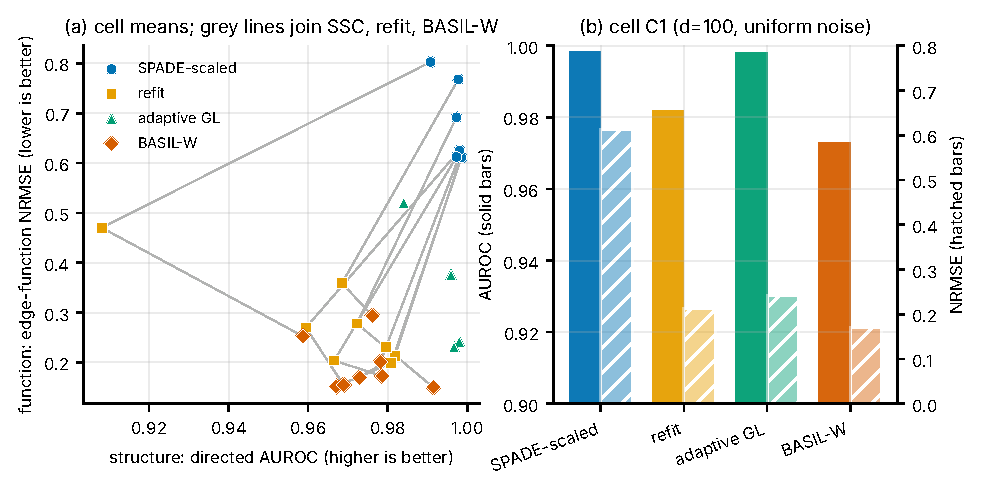
\includegraphics[width=\textwidth]{figures/fig1_structure_vs_function.pdf}
\caption{Structure versus function. (a) Cell means of directed AUROC (x) and edge-function NRMSE (y) for SPADE-scaled, refit, adaptive group lasso (only the four cells of the adaptive arm) and BASIL-W; grey lines join SSC, refit and BASIL-W within a cell. The learner with the best structure has the worst functions. (b) Both metrics in cell C1.}
\label{fig:s-vs-f}
\end{figure}

\begin{figure}[t]
\centering
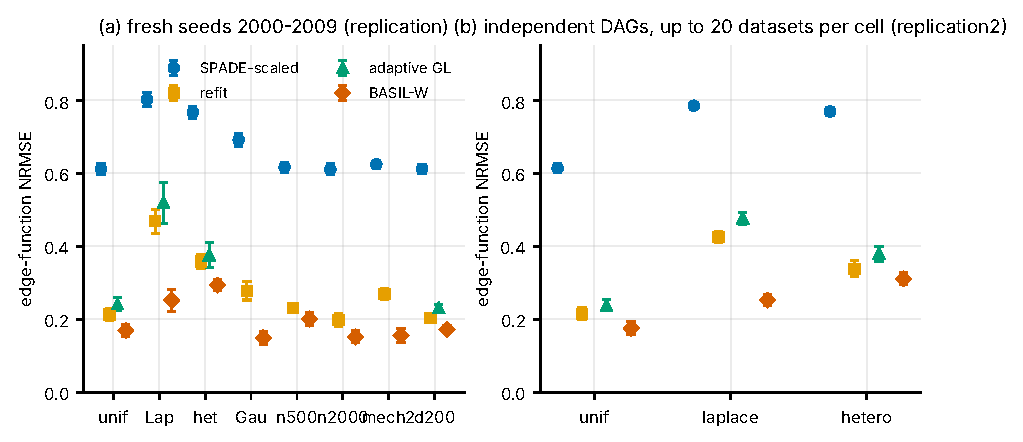
\includegraphics[width=\textwidth]{figures/fig2_edge_nrmse_by_cell.pdf}
\caption{Edge-function NRMSE by cell, with 95\% bootstrap intervals over datasets. The adaptive group lasso was run only in C1, C2, C3 and C8 and on a subset of datasets in C2, C3 and C8 (Table~\ref{tab:adaptive}). A second panel appears when the independent-DAG replication (Section~\ref{sec:rep2}) has been run.}
\label{fig:nrmse}
\end{figure}

\begin{figure}[t]
\centering
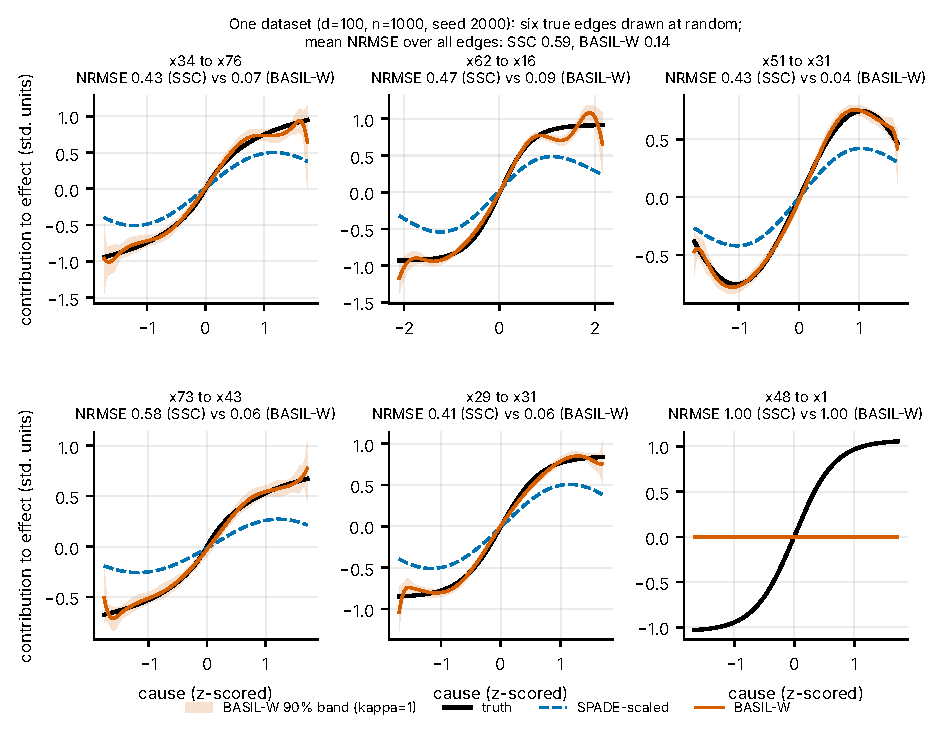
\includegraphics[width=\textwidth]{figures/fig3_example_curves.pdf}
\caption{Recovered curves on one dataset ($d=100$, $n=1000$, uniform noise, seed 2000). Black: truth; dashed blue: SPADE-scaled; orange: BASIL-W with its 90\% band ($\kappa=1$). The six edges were drawn at random, not selected on any result; the figure illustrates the amplitude shrinkage and, in the last panel, an edge missed by both methods (NRMSE 1); it is not evidence beyond the tables. Data: \texttt{data/example\_curves.npz}.}
\label{fig:curves}
\end{figure}

\paragraph{BASIL-W versus the refit.} BASIL-W has a lower mean NRMSE than the refit in all seven $d=100$ cells and the pre-registered tie criterion (BASIL-W $\le$ refit $+0.03$) holds in 7 of 7. It is significantly better after Holm correction (p = 0.014) only in C2 (Laplace, $-0.22$), C3 (heteroscedastic, $-0.065$), C4 (Gaussian, $-0.13$) and C7 (mechanism family 2, $-0.115$). In C1, C5 and C6 (uniform noise at $n=1000$, 500, 2000) the differences are $-0.043$, $-0.030$, $-0.047$, 6--8 of 10 datasets favour BASIL-W, and the supported statement is a tie within about 0.05, not superiority. The refit is fragile under heavy-tailed noise: under Laplace noise its AUROC falls to 0.908 (SSC 0.991) and its NRMSE is 0.47.

\paragraph{Pre-registered hypotheses.} Appendix~\ref{app:hyp} lists the verdicts. In short: the edge-function (H1) and do-effect (H3) hypotheses were confirmed in all cells; H2 (BASIL-W within 0.03 of the refit) was confirmed; H4 (AUROC loss at most 0.03) missed its target in two cells by 0.002 and 0.001, and the coverage part of H5 failed in seven of eight cells.

\subsection{Structure cost and calibration}
\label{sec:struct}

\begin{table}[t]
\centering
\caption{Structure, interventional-effect error and calibration by cell (means over datasets).}
\label{tab:struct}
\begin{adjustbox}{max width=\textwidth}
\begin{tabular}{lrrrrrrccrr}
\toprule
Cell & AUROC SSC & refit & BASIL-W & orient. SSC & refit & BASIL-W & do direct & do indirect & cover. & ECE \\
\midrule
C1 & 0.998 & 0.982 & 0.973 & 0.95 & 0.92 & 0.94 & 0.60 / 0.19 / 0.15 & 0.86 / 0.26 / 0.22 & 0.793 & 0.0014 \\
C2 & 0.991 & 0.908 & 0.959 & 0.74 & 0.75 & 0.92 & 0.76 / 0.41 / 0.18 & 0.92 / 0.50 / 0.33 & 0.753 & 0.0024 \\
C3 & 0.998 & 0.968 & 0.976 & 0.89 & 0.84 & 0.95 & 0.73 / 0.32 / 0.20 & 0.93 / 0.54 / 0.48 & 0.781 & 0.0016 \\
C4 & 0.997 & 0.972 & 0.992 & 0.90 & 0.88 & 0.98 & 0.66 / 0.22 / 0.13 & 0.87 / 0.34 / 0.23 & 0.808 & 0.0008 \\
C5 & 0.998 & 0.980 & 0.978 & 0.95 & 0.92 & 0.95 & 0.60 / 0.21 / 0.18 & 0.86 / 0.30 / 0.27 & 0.798 & 0.0012 \\
C6 & 0.999 & 0.981 & 0.967 & 0.95 & 0.92 & 0.93 & 0.60 / 0.16 / 0.15 & 0.86 / 0.23 / 0.21 & 0.774 & 0.0016 \\
C7 & 0.998 & 0.959 & 0.969 & 0.91 & 0.90 & 0.94 & 0.59 / 0.22 / 0.15 & 0.82 / 0.31 / 0.27 & 0.742 & 0.0015 \\
C8 & 0.997 & 0.967 & 0.979 & 0.95 & 0.93 & 0.95 & 0.58 / 0.16 / 0.14 & 0.86 / 0.27 / 0.21 & 0.788 & 0.0006 \\
\bottomrule
\end{tabular}
\end{adjustbox}

\smallskip
{\footnotesize Means over datasets. do-effect NRMSE for up to 20 direct and 20 indirect true pairs per dataset (SSC / refit / BASIL-W). Coverage: pointwise coverage of the 90\% BASIL-W band over true edges, kappa = 1; ECE of the edge probabilities. BASIL-W AUROC is lower than SSC in 9 or 10 of 10 datasets in every $d=100$ cell.}

\end{table}

SSC has the best structure in every cell (AUROC 0.991--0.999). The refit loses 0.016--0.083 AUROC, with the largest loss under Laplace noise. BASIL-W loses 0.006--0.032 relative to SSC (cell means $-0.025,-0.032,-0.022,-0.006,-0.020,-0.031,-0.029,-0.019$ for C1--C8); it is lower than SSC in 9 or 10 of 10 datasets in every $d=100$ cell (Holm p = 0.014), so the loss is real, and two cells just exceed the 0.03 target. BASIL-W has the best orientation under non-uniform noise (e.g.\ Laplace 0.919 against 0.745 for SSC). Edge probabilities are well calibrated (ECE $\le 0.0024$). The 90\% band coverage is 0.74--0.81 (Table~\ref{tab:struct}; Section~\ref{sec:bands}). The cost of BASIL-W is 1.23--1.44 times that of SSC (median wall-clock; SSC 27--31 s and BASIL-W 36--43 s at $d=100$, $n=1000$), that of the refit 1.47--1.70 times.

\subsection{Interventional effects}
\label{sec:do}

\begin{figure}[t]
\centering
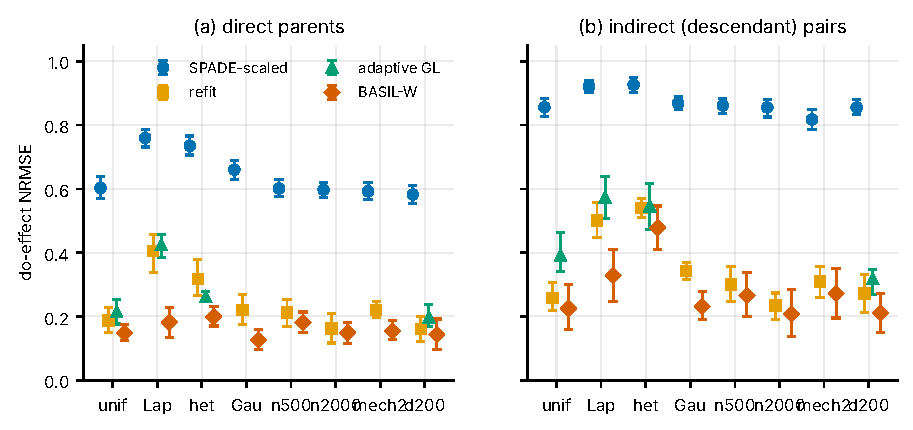
\includegraphics[width=\textwidth]{figures/fig4_do_effect.pdf}
\caption{Do-effect NRMSE for direct parents (a) and indirect (descendant) pairs (b), mean and 95\% bootstrap interval over datasets, by cell. SPADE-scaled's effects are wrong even for direct parents; the repaired models are much better, and refit and BASIL-W are close.}
\label{fig:do}
\end{figure}

Because SSC's curves are shrunken, the interventional-effect curves derived from them are wrong even for direct parents (NRMSE 0.58--0.76) and worse for indirect pairs (0.82--0.93), i.e.\ errors do not average out along paths but remain large. BASIL-W lowers the direct error by a factor of 3.3--5.3 relative to SSC (ratios 0.19--0.30) and the indirect error by 1.9--4.2 (ratios 0.24--0.52); heteroscedastic noise is the weakest case (indirect ratio 0.52). No dataset has an indirect BASIL-W error above 2 (0 of 75; the maximum is 0.69). Relative to the refit, BASIL-W's do-effects are lower in every cell mean but significantly so only in C2, C3, C4 and C7 for direct pairs (Holm p between 0.014 and 0.039), and only in C4 for indirect pairs (Holm 0.041); in C1, C5, C6 and C8 the two are statistically indistinguishable.

\subsection{The standard fix: adaptive group lasso}
\label{sec:adaptive}

\begin{table}[t]
\centering
\caption{Adaptive group lasso arm (SSA) on the replication seeds, with SSC, refit and BASIL-W taken from the replication runs on the same seeds.}
\label{tab:adaptive}
\begin{adjustbox}{max width=\textwidth}
\begin{tabular}{lrrrrrrrrrr}
\toprule
Cell & $N$ & SSC & SSA & refit & BASIL-W & SSA $-$ refit & SSA $-$ BASIL-W & p & AUROC SSA & AUROC BASIL-W \\
\midrule
d100 uniform & 10 & 0.612 & 0.241 & 0.213 & 0.169 & +0.029 (8/10) & +0.072 (10/10) & 0.002 & 0.998 & 0.973 \\
d100 Laplace & 5 & 0.805 & 0.520 & 0.470 & 0.261 & +0.049 (5/5) & +0.258 (5/5) & 0.062 & 0.984 & 0.953 \\
d100 hetero & 5 & 0.766 & 0.375 & 0.349 & 0.294 & +0.027 (4/5) & +0.082 (5/5) & 0.062 & 0.996 & 0.977 \\
d200 uniform & 3 & 0.606 & 0.230 & 0.193 & 0.176 & +0.037 (3/3) & +0.055 (3/3) & 0.250 & 0.997 & 0.977 \\
\bottomrule
\end{tabular}
\end{adjustbox}

\smallskip
{\footnotesize Adaptive group lasso (SSA: weights $(\|\theta\|+0.01)^{-1}$, same $\lambda=0.2/d$, $\gamma$ and $\epsilon$ not tuned) on the replication seeds; SSC, refit and BASIL-W values are the replication runs on the same seeds. Differences SSA minus comparator, in parentheses the number of datasets in which SSA is worse. Wilcoxon p (uncorrected) for SSA vs BASIL-W; with 5 or 3 datasets the minimum attainable p is 0.0625 or 0.25.}

\end{table}

Before the adaptive arm was run we predicted that SSA would land between SSC and the refit (NRMSE 0.3--0.5). It did better: at $d=100$ with uniform noise SSA has NRMSE 0.241 (slope 0.90), the same AUROC as SSC (0.998; orientation 0.950), and it is worse than BASIL-W by 0.072 (10 of 10 datasets, p = 0.002) and worse than the refit by 0.029 (8 of 10, p = 0.037). The SSA values at $d=200$ (0.230 against BASIL-W 0.176; three datasets), under heteroscedastic noise (0.375 against 0.294) and Laplace noise (0.520 against 0.261) show the same ordering (Table~\ref{tab:adaptive}). Read plainly: \emph{the standard adaptive group lasso closes about 85\% of the NRMSE gap between SPADE-scaled and BASIL-W at no structural cost}, and it is the only repair that preserves SSC's AUROC (BASIL-W loses 0.01--0.03, the refit more). BASIL-W's remaining advantage is small under uniform noise (0.055--0.072) and large under heavy tails (0.26), where the adaptive lasso is also much worse than at light tails. A practitioner who wants accurate curves and the best structure should therefore use the adaptive group lasso unless heavy-tailed noise or edge probabilities matter. The SSA runs were smaller than the replication (10, 5, 5 and 3 datasets); $\gamma$ and $\epsilon$ were not tuned, and a tuned adaptive lasso could narrow the gap further.

\subsection{Independent-DAG replication}
\label{sec:rep2}

The first replication uses 10 datasets per cell and shares graphs between cells. A second pre-registered replication with 20 datasets per cell, independent graphs per noise family and all four arms (SSC, SSA, refit, BASIL-W) is run in \texttt{research/replication2}. Table~\ref{tab:rep2} is generated from its results.

\begin{table}[t]
\centering
\caption{Independent-DAG replication (research/replication2).}
\label{tab:rep2}
\begin{adjustbox}{max width=\textwidth}
\begin{tabular}{lrrrrrrrrrrr}
\toprule
Noise & $N$ & SSC & SSA & refit & BASIL-W & BASIL-W $-$ SSA [95\% CI] & wins & Holm p & BASIL-W $-$ refit & BASIL-W$<$SSC \\
\midrule
uniform & 20 & 0.614 & 0.238 & 0.215 & 0.176 & -0.062 [-0.079, -0.046] & 19/20 & $<$0.001 & -0.039 (16/20) & 20/20 \\
Laplace & 20 & 0.786 & 0.477 & 0.426 & 0.253 & -0.224 [-0.239, -0.210] & 20/20 & $<$0.001 & -0.173 (20/20) & 20/20 \\
heteroscedastic & 20 & 0.770 & 0.379 & 0.338 & 0.311 & -0.068 [-0.082, -0.054] & 19/20 & $<$0.001 & -0.027 (14/20) & 20/20 \\
\bottomrule
\end{tabular}
\end{adjustbox}

\smallskip
{\footnotesize Independent-DAG replication (\texttt{research/replication2}): complete datasets only (all four arms present), edge-function NRMSE, mean over datasets. BASIL-W $-$ SSA: mean paired difference with 95\% bootstrap interval, number of datasets in which BASIL-W is lower, Holm-adjusted exact two-sided Wilcoxon p over the 9 pre-registered NRMSE tests (research/replication2/results/pairwise.csv). BASIL-W $-$ refit: mean difference (wins). Last column: datasets where BASIL-W $<$ SSC. The uniform seeds 3000--3012 coincide with the ablation datasets.}

\end{table}

\begin{table}[t]
\centering
\caption{Independent-DAG replication: structure, do-effects, calibration and cost.}
\label{tab:rep2b}
\begin{adjustbox}{max width=\textwidth}
\begin{tabular}{lccccccc}
\toprule
Noise & AUROC & do direct & do indirect & cover. (BASIL-W) & ECE & cost ratio \\
\midrule
uniform & 0.997 / 0.997 / 0.974 / 0.971 & 0.589 / 0.201 / 0.167 / 0.148 & 0.846 / 0.342 / 0.309 / 0.217 & 0.795 & 0.001 & 1.68 / 1.65 / 1.34 \\
\bottomrule
\end{tabular}
\end{adjustbox}

\smallskip
{\footnotesize Means over complete datasets (SSC / SSA / refit / BASIL-W). Cost: median over datasets of the per-dataset cost ratio to SSC (SSA / refit / BASIL-W), excluding metric code, shared loaded machine.}

\end{table}
\paragraph{Design.} $d=100$, $n=1000$, mechanism family 1; 20 datasets per cell and 60 in all, with their own DAGs, mechanism assignments and noise: seeds 3000--3019 (uniform), 3100--3119 (Laplace), 3200--3219 (heteroscedastic). All $60\times4$ runs completed, with no failures and no dataset with an indirect do-effect NRMSE above 2 for any arm. No parameter was retuned. Statistics as registered: exact Wilcoxon per cell, Holm adjustment over 3 cells $\times$ 3 pairs (BASIL-W vs SSC, BASIL-W vs SSA, SSA vs SSC; a separate Holm family for pairs with the refit), bootstrap intervals over datasets.

\paragraph{Verdicts against the plan.} \textbf{H1 (BASIL-W below SSC in at least 95\% of datasets per cell) is confirmed}: 20/20 in all three cells, with NRMSE ratios BASIL-W/SSC of 0.29 (uniform), 0.32 (Laplace) and 0.40 (heteroscedastic). \textbf{H2 (BASIL-W lower than SSA) is confirmed} and the kill criterion is not triggered: the SSA minus BASIL-W gaps are 0.062, 0.224 and 0.068, inside the predicted ranges, Holm $p=1.7\times10^{-5}$ in every cell, BASIL-W lower in 19/20, 20/20 and 19/20 datasets. Under uniform noise the gap is small in absolute terms (about 26\% of SSA's error) but consistent in sign. \textbf{H3 (SSA keeps SSC's AUROC within 0.005; BASIL-W loses 0.01--0.03) is only partly confirmed.} SSA minus SSC AUROC is $+0.0001$ (uniform) and $-0.0005$ (heteroscedastic), but $-0.0067$ under Laplace noise, which misses the 0.005 bound (Holm-significant, SSA lower in 20/20 datasets; small). BASIL-W minus SSC is $-0.023$, $-0.030$ and $-0.024$, inside the predicted range, with the Laplace value at its upper edge; BASIL-W is lower than SSC in 20/20, 20/20 and 19/20 datasets. \textbf{H4 (do-effect NRMSE BASIL-W $\le$ SSA $<$ SSC) is met on the cell means} in all cells for direct and indirect pairs, but the BASIL-W advantage over SSA is not established everywhere: for direct effects under uniform noise the difference is $-0.037$ [$-0.074$, $+0.007$], Holm $p=0.07$ (14/20 datasets favour BASIL-W), and for indirect effects under heteroscedastic noise it is $-0.063$ [$-0.119$, $+0.006$] with the interval including 0 (Holm $p=0.014$). Both are ties in practice. SSA is below SSC in every dataset and cell (20/20). H5 (cost, descriptive): median cost relative to SSC is 1.65, 1.65, 1.69 for SSA, 1.62, 1.69, 1.66 for the refit and 1.34, 1.35, 1.35 for BASIL-W (uniform, Laplace, heteroscedastic); on a loaded shared machine these ratios are $\pm30\%$ estimates.

\paragraph{BASIL-W against the refit is weak outside heavy tails.} The pooled picture over the 60 datasets (exploratory; graphs are independent across cells here) is BASIL-W minus SSA $-0.118$ [$-0.139$, $-0.098$], BASIL-W lower in 58/60; BASIL-W minus refit $-0.080$ [$-0.099$, $-0.061$], lower in 50/60. By cell, BASIL-W beats the refit by only 0.039 under uniform noise and 0.027 under heteroscedastic noise (Holm $p=0.003$ and $0.008$), and the refit has the lowest NRMSE of the four arms on 4/20 uniform and 6/20 heteroscedastic datasets (BASIL-W 15/20 and 14/20); only under Laplace noise is BASIL-W clearly better (0.173, 20/20). The adaptive group lasso is consistently a little worse than the plain refit on edge NRMSE (SSA minus refit $+0.023$, $+0.051$, $+0.041$; all Holm-significant). In cell means the adaptive group lasso closes about 85\% of the SSC-to-BASIL-W NRMSE gap in the uniform and heteroscedastic cells and 58\% under Laplace noise. These results do not support calling BASIL-W the best repair: it is the best of the four arms on average, with the advantage over the refit being practically small under light-tailed or heteroscedastic noise.

\paragraph{Comparison with the first replication.} Everything reproduces qualitatively on independent DAGs: signs, orderings and the structure result that SSA keeps SSC's AUROC. The BASIL-W advantage is somewhat smaller on the new data. The SSA gap shrank by 0.01--0.03 (0.062/0.224/0.068 against 0.072/0.258/0.082 earlier), and the BASIL-W minus refit difference under heteroscedastic noise fell from $-0.065$ (5 earlier datasets) to $-0.027$. Under uniform noise it is nearly unchanged ($-0.039$ against $-0.043$) and now significant after Holm correction. The earlier concern that the first replication reused DAGs across cells is addressed for the three noise families here, and the headline conclusions did not depend on those 10 graphs.

\paragraph{Calibration.} BASIL-W's 90\% bands cover 0.789, 0.761 and 0.757 of the true curve (uniform, Laplace, heteroscedastic) against the nominal 0.90, so the under-coverage found earlier persists; ECE of the edge probabilities is 0.0014--0.0021.

\paragraph{Caveats.} This is a replication of the experiment with the same generator, code family and hyperparameters, not an external validation; the three cells share mechanism family and density. The uniform seeds 3000--3012 coincide with the ablation validation and test datasets of Sections~\ref{sec:ablation} and~\ref{sec:bands}; no BASIL-W setting was changed by that work, but the uniform cell is not fully fresh. The adaptive group lasso used the untuned $\gamma=1$, $\epsilon=0.01$, which is the largest open threat to the BASIL-W-over-SSA result (Section~\ref{sec:adaptive2}). Direct do-effects of BASIL-W do not differ detectably from SSA under uniform noise (Holm $p=0.07$) or from the refit under uniform noise (Holm $p=0.43$). The datasets in a cell are independent, but there are only three noise families. Nothing is concluded here about real data, other generators, mechanism family 2, other $n$ or $d$, Gaussian noise or $d\ge200$. The plan had no deviations; one crash in \texttt{aggregate.py} (fewer than 3 complete datasets in a cell) was fixed without changing any statistic.


\subsection{Adaptive arm at \texorpdfstring{$d=500$}{d=500} and sensitivity to \texorpdfstring{$\gamma$ and $\epsilon$}{gamma and epsilon}}
\label{sec:adaptive2}

The adaptive arm was run only up to $d=200$ in the main grid. A pre-registered extension (\texttt{research/adaptive2}) runs it at $d=500$ (two datasets) and over a $3\times3$ grid of $(\gamma,\epsilon)$ at $d=100$ (five datasets) to test whether the gap to BASIL-W is an artefact of the untuned defaults.

\begin{table}[t]
\centering
\caption{Adaptive arm at $d=500$ and $(\gamma,\epsilon)$ sensitivity (research/adaptive2).}
\label{tab:adaptive2}

\bigskip
\textbf{(b) $(\gamma,\epsilon)$ grid, $d=100$, uniform, seeds 2000--2001.}

\begin{adjustbox}{max width=\textwidth}
\begin{tabular}{llrrrr}
\toprule
$\gamma$ & $\epsilon$ & $N$ & NRMSE & slope & AUROC \\
\midrule
0.5 & 0.001 & 2 & 0.196 & 0.92 & 0.999 \\
0.5 & 0.01 & 2 & 0.282 & 0.83 & 0.998 \\
0.5 & 0.1 & 2 & 0.333 & 0.80 & 0.999 \\
1 & 0.001 & 2 & 0.187 & 0.92 & 0.999 \\
1 & 0.01 & 2 & 0.200 & 0.92 & 0.999 \\
1 & 0.1 & 2 & 0.301 & 0.82 & 0.997 \\
2 & 0.001 & 2 & 0.195 & 0.93 & 0.999 \\
2 & 0.01 & 2 & 0.188 & 0.93 & 0.999 \\
2 & 0.1 & 2 & 0.219 & 0.92 & 0.999 \\
\bottomrule
\end{tabular}
\end{adjustbox}

\smallskip
{\footnotesize Reference on the same seeds (replication): SSC 0.592, refit 0.226, BASIL-W 0.164. The default $(1,0.01)$ is the configuration used for all headline numbers; the grid is a sensitivity analysis and no setting was selected.}

\end{table}
\paragraph{Part A: $d=500$ (two datasets, descriptive).} With $n=1000$, uniform noise, mechanism family 1 and seeds 1000 and 1001, the mean edge-function NRMSE is 0.690 for SSC, 0.295 for SSA ($\gamma=1$, $\epsilon=0.01$), 0.229 for the refit and 0.162 for BASIL-W (per seed SSA 0.308 and 0.282, BASIL-W 0.166 and 0.157). AUROC is 0.9983 (SSC), 0.9975 (SSA), 0.9534 (refit) and 0.9773 (BASIL-W); orientation 0.919, 0.919, 0.912 and 0.952. Re-run SSC and refit reproduce the earlier CSVs exactly, so the comparison is on identical models. The pre-registered predictions fared as follows. P1 (SSA NRMSE 0.22--0.30, next to the refit, worse than BASIL-W): inside the numerical range but at its top; SSA is 0.066 worse than the refit and 0.133 worse than BASIL-W, a larger gap than at $d=100$ and $200$ (+0.072 and +0.055 against BASIL-W), so SSA is not next to the refit. P2 (AUROC within 0.005 of SSC): met. \textbf{P3 (SSA do-effects between the refit and BASIL-W): not met.} Direct effects tie with the refit (0.19 against 0.19) and indirect effects are clearly worse (0.42 against 0.28 for the refit and 0.17 for BASIL-W), though far better than SSC (0.90). SSA's do-effects are therefore worse than the plain refit's, a failed prediction. P4 (fit time near the refit): met (about 250~s against 225--259~s). At $d=500$ the adaptive group lasso closes about 75\% of the SSC-to-BASIL-W gap, $(0.690-0.295)/(0.690-0.162)$, against about 85\% at $d=100$; the sentence about 85\% is specific to $d=100$. BASIL-W's fit time beyond the shared SPADE-scaled fit is smaller (69~s, one dataset) than either refit; BASIL-W seed 1001 values come from an earlier independent run on the same data.

\paragraph{Part B: $(\gamma,\epsilon)$ grid (five datasets, sensitivity only).} At $d=100$, uniform noise, seeds 2000--2004, the mean NRMSE over the nine settings ranges from 0.199 to 0.359, a spread of 0.16 (the default 0.234, per-dataset 0.210, 0.191, 0.211, 0.297, 0.260). The registered expectation of a spread below 0.05 (Q1) failed: $\epsilon=0.1$ is clearly worse (0.245--0.359) at every $\gamma$, consistent with a large $\epsilon$ flattening the weights towards a plain group lasso; the cell $(0.5,0.01)$ at 0.318 is worse than both its neighbours in $\epsilon$ and the pattern is not smooth in $\gamma$, which five datasets cannot resolve. AUROC is 0.9978--0.9988 in all nine settings, so structure is insensitive to $\gamma$ and $\epsilon$; the expectation that $\gamma=2$ with small $\epsilon$ loses AUROC failed (it has the highest, 0.9988). No setting reaches BASIL-W (0.159 on these seeds; rule: at most 0.169): the best grid mean, $(1,0.001)$ at 0.199, is still 0.040 above (Q3 confirmed). Two settings beat the default by more than 0.03 on the mean and on 5/5 datasets, $(1,0.001)$ by 0.035 and $(2,0.01)$ by 0.030. By the pre-registered rule they are ``clearly better'' in this sample, but they were examined on the same seeds used for the sensitivity analysis, and the default had already been run on seeds 2000--2004. \textbf{They are not adopted}: the default $(1,0.01)$ remains the SSA configuration for every headline number. If an improved setting is wanted, the two candidates should be validated against the default on fresh seeds with the choice and threshold written first.

\paragraph{What this changes.} The statement that $\gamma$ and $\epsilon$ were untuned can now be accompanied by a sensitivity result: structure does not depend on them, edge-function error does (0.20--0.36, mainly through $\epsilon$), and a smaller $\epsilon$ or $\gamma=2$ would likely shrink SSA's gap to BASIL-W at $d=100$ by roughly a quarter to a third without closing it. The claim that BASIL-W has lower NRMSE than the adaptive group lasso holds in every grid setting at $d=100$ (on means), but this does not remove the tuning threat, because the grid is five datasets, one noise family and one mechanism family, and the grid seeds cannot select a setting.

\paragraph{Limitations.} Two datasets at $d=500$ (BASIL-W time from one), five for the grid, no significance claims, one generator family, uniform noise and mechanism family 1 only; wall-clock times on a loaded shared machine.


\subsection{Ablations}
\label{sec:ablation}

\begin{table}[t]
\centering
\caption{BASIL-W ablations: one change at a time ($d=100$, $n=1000$, uniform noise, 8 test datasets).}
\label{tab:ablation}
\begin{adjustbox}{max width=\textwidth}
\begin{tabular}{lrrrrrrrrr}
\toprule
Variant & NRMSE & $\Delta$ & orient. & $\Delta$ & AUROC & do indirect & cover. & gap & time \\
\midrule
BASIL-W (reference) & 0.177 & -- & 0.943 & -- & 0.971 & 0.248 & 0.798 & 8.8 & 10.8 \\
candidates by marginal $R^2$ & 0.176 & -0.001 & 0.943 & +0.000 & 0.972 & 0.251 & 0.798 & 17.8 & 10.6 \\
cold start (random order) & 0.324 & +0.147 & 0.809 & -0.133 & 0.909 & 0.548 & 0.678 & 543.0 & 9.6 \\
cold start + $R^2$ candidates (BASIL-S) & 0.318 & +0.141 & 0.821 & -0.121 & 0.921 & 0.593 & 0.697 & 575.9 & 10.0 \\
$g=n/4$ & 0.176 & -0.001 & 0.945 & +0.002 & 0.972 & 0.251 & 0.801 & 15.7 & 10.3 \\
$g=4n$ & 0.176 & -0.001 & 0.942 & -0.000 & 0.974 & 0.253 & 0.799 & 65.6 & 10.7 \\
$\pi \times 0.5$ & 0.177 & -0.000 & 0.943 & +0.000 & 0.972 & 0.248 & 0.798 & 7.5 & 10.0 \\
$\pi \times 2$ & 0.176 & -0.002 & 0.945 & +0.002 & 0.973 & 0.251 & 0.800 & 17.1 & 10.3 \\
$k_{max}=2$ & 0.280 & +0.103 & 0.894 & -0.048 & 0.951 & 0.422 & 0.706 & 85.4 & 6.9 \\
4 chains, $600d$ iterations & 0.173 & -0.004 & 0.934 & -0.009 & 0.974 & 0.227 & 0.807 & 30.9 & 23.5 \\
\bottomrule
\end{tabular}
\end{adjustbox}

\smallskip
{\footnotesize d=100, n=1000, uniform noise, 8 test datasets (seeds 3005--3012), one change at a time. $\Delta$ = paired mean difference to the reference. End-score gap: max$-$min over chains of the mean log-score at the end of the chains (nats); time: BASIL fit only, 1 core, seconds. No significance tests.}

\end{table}

Table~\ref{tab:ablation} summarises the ablations. The warm start from SSC's order is essential: a cold start raises NRMSE from 0.177 to 0.324 and lowers orientation from 0.943 to 0.809 (8 of 8 datasets worse), because cold chains do not converge in $200d$ iterations (end-score gaps of hundreds of nats); longer cold chains were not run, so this is a statement about this chain length. The source of the candidate set does not matter at $d=100$ (candidate recall is 1.000 with either ranking), and the prior scale $g$ and inclusion prior $\pi$ are robust ($|\Delta\NRMSE|\le0.002$). Capping the parent set at $k_{\max}=2$ is harmful ($+0.103$ NRMSE, 8 of 8 worse; with mean degree 2 a non-trivial share of nodes have three or more parents). Four chains of $600d$ iterations change NRMSE by $-0.004$ and indirect do-effect NRMSE from 0.248 to 0.227, but the chain end-score gap does not shrink (31 nats against 8.8), so the chains are not provably converged; the default is adequate for edge-function NRMSE and not demonstrably so for indirect effects. Variants that keep the warm start all look alike, so BASIL-W's output here is largely determined by SSC's order and candidates plus local refinement; what happens when SSC's order is poor was not tested. Three registered predictions were wrong (the size of the warm-start effect, the effect of $k_{\max}=2$ and chain convergence).

\subsection{Credible bands}
\label{sec:bands}

\begin{table}[t]
\centering
\caption{Band coverage before and after variance inflation, test datasets.}
\label{tab:bands}
\begin{adjustbox}{max width=\textwidth}
\begin{tabular}{llrrrrr}
\toprule
Noise (datasets) & $\kappa$ & all edges & found & missed & whole curve & mean width \\
\midrule
uniform (8) & 1 & 0.798 & 0.877 & 0.095 & 0.15 & 0.140 \\
uniform (8) & 1.55 & 0.894 & 0.981 & 0.112 & 0.61 & 0.216 \\
Laplace (5) & 1 & 0.796 & 0.850 & 0.207 & 0.05 & 0.141 \\
Laplace (5) & 1.55 & 0.904 & 0.964 & 0.249 & 0.32 & 0.219 \\
hetero (5) & 1 & 0.790 & 0.835 & 0.304 & 0.03 & 0.174 \\
hetero (5) & 1.55 & 0.908 & 0.960 & 0.357 & 0.23 & 0.269 \\
\bottomrule
\end{tabular}
\end{adjustbox}

\smallskip
{\footnotesize Pointwise coverage of the 90\% band (5th/95th percentile of $m+\kappa(D-m)$ for posterior draws $D$ and mean $m$) over true edges, mean over datasets (found/missed: pooled over edges). $\kappa^*=1.55$ was chosen as the smallest value reaching coverage 0.90 on 5 validation datasets (seeds 3000--3004) and frozen. `found' = posterior inclusion $P>0.9$; `missed' = $P\le0.9$; `whole curve' = share of curves entirely inside the band.}

\end{table}

\begin{figure}[t]
\centering
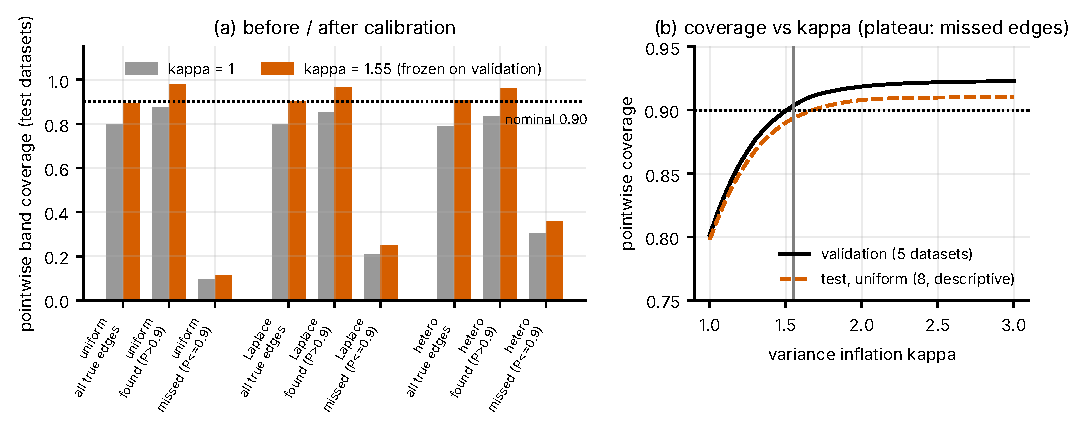
\includegraphics[width=\textwidth]{figures/fig6_band_coverage.pdf}
\caption{Coverage of 90\% bands before ($\kappa=1$) and after ($\kappa=1.55$, frozen on validation) calibration. (a) By noise family and by whether the edge was found; (b) coverage as a function of $\kappa$ on validation and, for description only, on the uniform test datasets.}
\label{fig:bands}
\end{figure}

On five validation datasets the bands at $\kappa=1$ cover 0.802 of the truth pointwise (nominal 0.90); only 11\% of the curves lie entirely inside the band. The diagnosis is that 72\% of the shortfall comes from the 8\% of true edges the model does not find ($P\le0.9$): their band is a spike of width 0.03 around zero while the truth is not zero. For found edges the shortfall is small (0.87 against 0.90), $z$-scores are centred (mean $-0.004$, sd 1.03), and the noise variance, shrinkage and spline-approximation error are ruled out as main causes. We therefore tried a single remedy, posterior-variance inflation $m+\kappa(D-m)$. The smallest $\kappa$ with validation coverage $\ge0.90$ is $\kappa^\ast=1.55$ (frozen), which gives test coverage 0.894, 0.904 and 0.908 for uniform, Laplace and heteroscedastic noise with bands 1.55 times wider (Table~\ref{tab:bands}). This is average validity obtained partly for the wrong reason: found edges are over-covered (0.96--0.98 instead of 0.90) while missed edges remain uncovered (0.11--0.36), and the whole-curve (simultaneous) coverage is only 0.61 (uniform). The per-dataset coverage ranges from 0.78 to 0.93 for the uniform test datasets at $\kappa^\ast$ because the share of missed edges was 16\% on test and 8\% on validation; $\kappa^\ast$ was somewhat lucky and about 1.7--2.0 would have been needed on the test sets to reach 0.90. We conclude that edge probabilities (ECE $\le0.0024$) are calibrated, curve bands are not conditionally valid, and that the honest remedy for missed edges is a better structure estimate. Split-conformal and bootstrap alternatives were not implemented.

\subsection{Semi-synthetic benchmark from Sachs}
\label{sec:semisyn}

Real data have no function ground truth. A semi-synthetic design fits a model to the Sachs data and simulates from the fitted SEM, so that edge functions are known while the graph and the functional shapes are of empirical origin (\texttt{research/semisyn}).

\begin{table}[t]
\centering
\caption{Semi-synthetic Sachs benchmark (research/semisyn).}
\label{tab:semisyn}
\begin{adjustbox}{max width=\textwidth}
\begin{tabular}{rrllrrrrrrrll}
\toprule
$d$ & $n$ & Noise & $N$ & SSC & SSA & refit & BASIL-W & GAM-ridge & ratio & AUROC SSC / BASIL-W & cover. \\
\midrule
11 & 2000 & bootstrap residuals & 20 & 0.826 & 0.711 & 0.730 & 0.391 & 0.394 & 0.47 & 0.821 / 0.893 & 0.52 \\
11 & 2000 & Gaussian & 20 & 0.714 & 0.495 & 0.516 & 0.283 & 0.362 & 0.40 & 0.860 / 0.993 & 0.63 \\
11 & 500 & bootstrap residuals & 20 & 0.835 & 0.741 & 0.759 & 0.652 & 0.539 & 0.78 & 0.817 / 0.837 & 0.39 \\
11 & 500 & Gaussian & 20 & 0.721 & 0.563 & 0.586 & 0.585 & 0.530 & 0.81 & 0.856 / 0.965 & 0.45 \\
110 & 2000 & bootstrap residuals & 5 & 0.930 & 0.820 & 0.757 & 0.398 & -- & 0.43 & 0.957 / 0.919 & 0.53 \\
\bottomrule
\end{tabular}
\end{adjustbox}

\smallskip
{\footnotesize Semi-synthetic Sachs benchmark (research/semisyn; 17 true edges on 11 nodes, ten copies at $d=110$): edge-function NRMSE, mean over datasets. Ratio: mean of per-dataset BASIL-W/SSC. Coverage: 95\% band of BASIL-W over true curves. GAM-ridge did not finish at $d=110$. At $d=11$ SSC and plain SPADE are identical. The truth is a fitted model of contested data.}

\end{table}
\paragraph{Status.} \textbf{PENDING.} At build time \nSemiDone{} semi-synthetic datasets were available; no conclusion is drawn.


\subsection{Real data: Sachs}
\label{sec:sachs}

\begin{figure}[t]
\centering
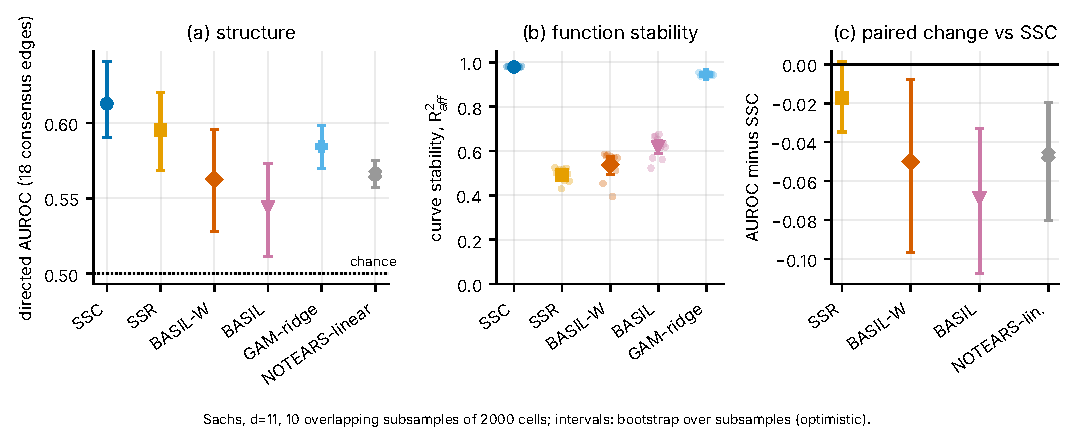
\includegraphics[width=\textwidth]{figures/fig5_sachs.pdf}
\caption{Sachs data ($d=11$, 10 overlapping subsamples of 2000 cells). (a) Directed AUROC against the 18 consensus edges; (b) stability of edge curves across subsamples on a common edge set (an unselected edge counts as zero); (c) paired AUROC change relative to SPADE-scaled. Intervals are bootstrap over subsamples and optimistic.}
\label{fig:sachs}
\end{figure}

\begin{table}[t]
\centering
\caption{Sachs: structure and function stability (10 subsamples).}
\label{tab:sachs}
\begin{adjustbox}{max width=\textwidth}
\begin{tabular}{lrrrrrr}
\toprule
Method & AUROC [95\% CI] & AUPRC & skel. AUROC & orient. & hits in top 18 & stability \\
\midrule
SSC (SPADE-scaled) & 0.613 [0.590, 0.641] & 0.291 & 0.690 & 0.51 & 5.8 & 0.98 \\
refit & 0.595 [0.568, 0.621] & 0.266 & 0.688 & 0.53 & 6.1 & 0.49 \\
BASIL-W & 0.563 [0.528, 0.596] & 0.248 & 0.703 & 0.58 & 5.8 & 0.54 \\
BASIL (full) & 0.544 [0.511, 0.573] & 0.227 & 0.683 & 0.51 & 5.3 & 0.62 \\
GAM-ridge & 0.584 [0.570, 0.599] & 0.287 & 0.735 & 0.40 & 6.1 & 0.94 \\
NOTEARS-linear & 0.566 [0.557, 0.575] & 0.239 & 0.634 & 0.53 & 5.0 & -- \\
DAGMA-linear & 0.435 [0.416, 0.450] & 0.168 & 0.688 & 0.31 & 3.0 & -- \\
var-sortnregress (z-scored) & 0.503 [0.460, 0.545] & 0.207 & 0.664 & 0.44 & 3.3 & -- \\
\bottomrule
\end{tabular}
\end{adjustbox}

\smallskip
{\footnotesize Sachs, $d=11$, 10 subsamples of 2000 cells (overlapping, so intervals are optimistic), 18 consensus edges (contested; chance AUPRC 0.164, about 2.9 hits at chance). Stability: mean R$^2_{aff}$ of the edge curves across subsamples on the 24 edges that are in SSC's top 18 in at least 3 subsamples; an unselected edge counts as a zero curve (R$^2=0$), which is what drives the low values for refit and BASIL-W.}

\end{table}

On the Sachs flow-cytometry data (7466 cells, $d=11$, natural log then z-score; 10 subsamples of 2000 cells; 18 consensus edges, \citealt{sachs2005}) no repair improves structure (Table~\ref{tab:sachs}, Figure~\ref{fig:sachs}). AUROC is 0.613 for SSC, 0.595 for the refit, 0.563 for BASIL-W and 0.544 for full BASIL; orientation is about 0.5 for every method. SSC places 5.8 true edges in its top 18 on average, against about 2.9 expected at chance. Relative to SSC the refit passes the pre-registered ``no loss'' rule ($-0.017$); BASIL-W ($-0.050$) and full BASIL ($-0.069$) lose more than 0.03, and SSC beats linear NOTEARS by 0.047 AUROC. Function stability across subsamples on a common set of 24 edges is 0.98 for SSC, 0.54 for BASIL-W and 0.49 for the refit; the difference is selection instability: the refit and BASIL-W return a zero curve for about 35\% of (edge, subsample) cells, SSC never does, and when an edge is kept in both subsamples all methods are stable (R$^2_{aff}$ 0.96--0.98). By the pre-registered rule the refit and BASIL-W are therefore ``less stable'' than SSC. The amplitude of the repaired curves relative to SSC is 1.60 (refit) and 1.41 (BASIL-W), i.e.\ the shrinkage predicted by the simulations is present but smaller than the factor of about 2.3 that the synthetic slope would imply, and there is no ground truth to say which amplitude is right. Sign sanity checks against three textbook relations were uninformative or unsupportive. This is a negative result for using the repairs as-is on real data. High stability of SSC reflects in part that it is a smooth always-on fit; stability is not correctness and not evidence of causal meaning (only two of the six top SSC edges are consensus edges in the consensus direction).

\subsection{Negative results}
\label{sec:neg}

\begin{table}[t]
\centering
\caption{Negative and failed results kept in the paper.}
\label{tab:neg}
\begin{adjustbox}{max width=\textwidth}
\begin{tabular}{p{2.9cm}p{3.2cm}p{6.2cm}p{2.6cm}}
\toprule
Attempt & Setting & Outcome & Verdict \\
\midrule
SPIRE (group-MCP + HSIC term) & $d=10$, $n=1000$, 30 datasets & AUROC $-0.021$ [$-0.031,-0.010$] vs SPADE; slope 0.75 (kill line 0.80); HSIC term adds $+0.05$ orientation at best, not significant on validation & H1 fails, H2 inconclusive \\
BASIL-S cold start & $d=100$--$500$, 5 datasets (1 at $d=500$) & chain end-scores differ by hundreds of nats; AUROC $-0.02$ to $-0.03$ vs SPADE-scaled; orientation 0.83 vs 0.94 at $d=200$ (original); $d=500$: orientation 0.71, slope 0.51 & does not scale as specified \\
BASIL-S, cold start (ablation) & $d=100$, 8 datasets & NRMSE 0.324 vs 0.177, orientation 0.809 vs 0.943 (8/8 worse) & warm start essential \\
Full BASIL & $d=50$ & about 11 min per dataset; no better than BASIL-W on Sachs (AUROC 0.544) & not scalable \\
SCORE / NoGAM & $d=10$, 10 datasets & AUROC 0.858 / 0.895 vs 0.980 (SPADE), 5--10$\times$ slower & baseline only \\
Pre-registered BASIL-W do-effects & $d\ge100$, 4 of 45 datasets & indirect do-effect NRMSE up to 185 (coefficients up to $1.4\times10^7$); fixed post hoc by a ridge map & instability; fixed, 0/75 on fresh seeds \\
\bottomrule
\end{tabular}
\end{adjustbox}

\smallskip
{\footnotesize Numbers from research/spire (README\_results, README\_basil, README\_scale, README\_do), research/ablation and research/real\_data.}

\end{table}

Table~\ref{tab:neg} collects the attempts that did not work. Three deserve a sentence each.

\paragraph{SPIRE.} The first idea of the project was a single objective: a group-MCP penalty, which has no shrinkage on strong edges by construction, plus a residual-independence (HSIC) term to exploit the ANM identifiability signal. At $d=10$ with 30 test datasets it lost 0.021 AUROC against SPADE and reached a slope of 0.75 (kill line 0.80) while the old adaptive heuristic reached 0.93 without an AUROC loss; the HSIC term added at most 0.05 orientation and was not significant on validation. The suspected reason is that exact zeros from the proximal step discard ranking information that SPADE's dense soft fit keeps; this is a hypothesis, and a convergence-budget test did not change the result. The independence-plus-adaptive-group-sparsity idea is also pursued by \citet{yao2026}.

\paragraph{BASIL-S and full BASIL.} Full BASIL took about 11 minutes per dataset at $d=50$. The screened variant BASIL-S was 57 times faster at $d=50$ and passed its faithfulness criterion, but with random starts its two chains disagreed by hundreds to thousands of nats at $d\ge100$, orientation collapsed at $d=200$ (0.830 against 0.942 for SPADE-scaled), and at $d=500$ (one dataset) orientation was 0.714 and the slope 0.51. An amended version (greedy initialisation, 3$\times$ longer chains, chain selection) was developed on validation seeds and recovered orientation but not AUROC (still 0.02--0.03 below) and was no faster than SPADE-scaled at $d=200$. SPADE-scaled itself already scales (AUROC 0.997--0.999 at $d=100$, 200, 500; 0.7--9 minutes per dataset), so scalability is not a differentiator for BASIL. The solution that works (BASIL-W) starts from SPADE-scaled's order, which makes it a refinement of the learner, not an independent estimator.

\paragraph{Numerical instability of the pre-registered do-effects.} Four of 45 pre-registered BASIL-W datasets gave indirect do-effect NRMSE far above 1 (up to 185). The cause, diagnosed on one case, was coefficients up to $1.4\times10^7$ in the whitened-to-spline coefficient map along weakly excited spline directions, which makes propagated interventions leave the data support. A ridge-stabilised map removed it (0 of 75 datasets above NRMSE 2 on fresh seeds; Section~\ref{sec:do}). The stabilisation was chosen after seeing test results, with a single value of its constant, and confirmed on fresh seeds.\label{sec:do-instab}

\paragraph{Other.} SCORE and NoGAM are 0.07--0.11 AUROC below SSC at $d=10$ and 5--10 times slower; the GAM-ridge baseline without DAG constraint has similar skeleton AUROC to SPADE but orientation 0.29 lower (0.65 against 0.95), so the DAG constraint matters for orientation, not for the skeleton.

%=====================================================================
\section{Discussion and limitations}
\label{sec:discussion}

\paragraph{What the evidence supports.} (i) Structure-accurate sparse spline learners can return edge functions with less than half of the true amplitude at $d$ up to 500, across noise families, sample sizes and two mechanism families, and this carries over to interventional effects. (ii) The cheap fixes work: the adaptive group lasso removes most of the error without changing the selected structure, and the refit removes about two thirds of it at a structural cost. (iii) A Bayesian model-averaged estimator warm-started from the learner's order removes somewhat more, is more robust to heavy tails and heteroscedasticity than the refit, and supplies calibrated edge probabilities, at the price of AUROC and a more complex pipeline. We do not recommend BASIL-W over the adaptive group lasso as a default.

\paragraph{Limitations (complete list).}
\begin{enumerate}[leftmargin=*,itemsep=2pt]
  \item Simulation is the only place where function ground truth exists; the real-data evidence is negative or ambiguous, and the semi-synthetic benchmark (Section~\ref{sec:semisyn}) inherits the assumptions of the fitted model.
  \item Ten datasets per cell in the first replication, with cells C1--C6 sharing the same 10 DAGs, so pooled p-values overstate the evidence; the independent-DAG replication has 20 datasets per cell and three noise families only.
  \item A single generator family (iSCM with Erd\H{o}s--R\'enyi graphs of expected degree 2, two mechanism families, four noise types); no other graph densities, scale-free graphs, non-additive mechanisms, latent confounding or measurement error; mechanism functions are smooth and low-order.
  \item $d=500$ rests on two datasets and, in the first grid, on the BASIL-W version before stabilisation; the adaptive arm at $d=500$ is also two datasets (Section~\ref{sec:adaptive2}).
  \item The ridge stabilisation of BASIL-W's do-effects was chosen after seeing test results with one value of its constant; it was confirmed on fresh seeds (0 of 75 explosions) but never tuned.
  \item The adaptive group lasso used a single untuned setting of $\gamma$ and $\epsilon$ in the main grid, and was run on 3--10 datasets per cell; the sensitivity study is small (five datasets, no significance claims).
  \item The novelty of the repairs is limited (Section~\ref{sec:novelty}); the literature check relied on web search and abstract-level reading. The concurrent ICML 2026 paper \citep{yao2026} was read via its abstract only; \citet{kuskova2026} likewise.
  \item Credible bands are valid only on average: the calibration constant $\kappa^\ast$ was chosen on five validation datasets and was somewhat lucky; found edges are over-covered, missed edges remain uncovered; simultaneous coverage is low.
  \item BASIL-W inherits its candidate set and its starting order from SPADE-scaled; if SPADE-scaled's order is poor, BASIL-W's behaviour is untested. Chains are not provably converged: four chains do not agree better than two.
  \item BASIL-W's AUROC is below SPADE-scaled's in essentially every dataset (0.006--0.032 on average) and two cells miss the pre-registered 0.03 target by 0.001--0.002.
  \item The Sachs consensus graph is contested, the data pool interventional conditions that the methods do not use, $d=11$ with 18 edges makes 0.05 AUPRC about one edge, the 10 subsamples overlap by about 27\% (intervals optimistic), and there is no ground truth for the functions. The three sign-sanity relations were taken from memory of the standard cascade and not verified against the original text.
  \item Order MCMC has a prior bias towards graphs compatible with many orders \citep{viinikka2020}, which we do not correct; the Gaussian likelihood and $k_{\max}=3$ limit BASIL-W; model errors, not sampler errors, dominate in some datasets (the true order scored 25--46 nats below the MCMC order on an early validation dataset).
  \item The refit multiplier $k=1.5$ was tuned on three validation datasets and exploits that the generating graphs have mean degree 2; a user may not know the density. Refit and adaptive baselines were given the screened candidates and $\lambda=0.2/d$ of SPADE-scaled, whose constants were fixed on an earlier generator.
  \item The BASIL-W ablations are on 8 datasets without significance tests, and three registered predictions were wrong.
  \item Cost ratios were measured on a shared, loaded machine and may not transfer; the 4-core CPU timings exclude metric code.
  \item Some of the independent-DAG replication's uniform datasets (seeds 3000--3012) coincide with the seeds used for the band-calibration and ablation work at $d=100$ (validation 3000--3004, test 3005--3012); no BASIL-W setting was changed by that work, but those datasets are not untouched (Section~\ref{sec:rep2}).
  \item Do-effect evaluation covers single-node hard interventions on a 15-point grid and at most 20 direct and 20 indirect pairs per dataset; pairs with tiny true effects are skipped (about 10\% of pairs, identical across methods).
\end{enumerate}

\paragraph{Risks of misreading.} The largest NRMSE reductions are relative to a learner (SPADE-scaled with $\lambda=0.2/d$) that is deliberately sparse; a less sparse baseline would shrink less. Our result is about the shape bias of sparse group-penalised fits, not about any specific software.

%=====================================================================
\section{Conclusion}
\label{sec:conclusion}
Finding the edges is not enough: on iSCM data a screened group-lasso spline learner has near-perfect structure but returns curves with about 44\% of the true amplitude, and its interventional effects are wrong even for direct parents. Standard repairs work. The adaptive group lasso gets most of the way without hurting structure; a refit gets two thirds of the way at a structural cost and breaks down under heavy-tailed noise; a warm-started Bayesian model average goes a little further, is more robust, and adds calibrated edge probabilities, but costs AUROC, has under-covering bands and, on the one real dataset we could test, is less stable than the unrepaired learner. Reporting edge-function error next to structure metrics costs little and changes the ranking of methods. The evidence is simulation-based with one generator family and small cell sizes; the real-data evidence is negative.

%=====================================================================
\section*{Reproducibility statement}
\label{sec:repro}
\textbf{Code and data.} All code, plans, raw per-dataset CSVs and analysis scripts are in the git repository, under \texttt{research/} (repository location and release commit: \placeholder{to be inserted by the authors at release}). Datasets are generated from seeds by \texttt{bench.gen\_full}; the Sachs data are in \texttt{data/sachs/} (7466 cells, 11 variables, consensus graph with 18 edges). \textbf{Regenerating this paper.} From \texttt{research/paper/ms/}: \texttt{python3.13 make\_example\_curves.py} (about two minutes, one core), \texttt{python3.13 make\_figures.py}, \texttt{python3.13 make\_tables.py}, then \texttt{pdflatex main; bibtex main; pdflatex main; pdflatex main}. \textbf{Re-running the experiments.} Each experiment directory has a job list and runner: for example \texttt{research/replication/run\_all.sh} followed by \texttt{python3.13 aggregate.py}; the replication of 75 datasets takes several hours on 2 jobs of a 4-core CPU. \textbf{Seeds.} Validation 0--9 and 3000--3004; earlier tests 1000--1004 and 1000--1029 ($d=10$); confirmatory 2000--2009 (C8: 2000--2004); ablation tests 3005--3012; Sachs subsamples seeds 0--9 (\texttt{RandomState(r).choice(7466, 2000)}); method seed 0 everywhere. One bit-identical re-run check on two datasets confirmed that the replication code reproduces the earlier numbers. \textbf{Hardware and software.} CPU only, a shared 4-core machine (no GPU), one thread per job, at most two parallel jobs; Python 3.13, PyTorch, NumPy, scikit-learn, SciPy. Timings are noisy.

%=====================================================================
\section*{Declarations}
\paragraph{Author contributions.} \placeholder{To be completed by the authors, e.g.\ following the CRediT taxonomy.}
\paragraph{Competing interests.} \placeholder{To be completed by the authors.}
\paragraph{Funding.} \placeholder{To be completed by the authors.}
\paragraph{Data availability.} \placeholder{To be completed by the authors. Synthetic data are generated by the released code from stated seeds; the Sachs data are a public benchmark (source and licence to be stated).}
\paragraph{Use of AI assistance.} \placeholder{Placeholder to be reviewed and adapted by the authors to the target venue's policy. Facts: an AI assistant (Claude, Anthropic) was used to write code, run experiments, analyse results and draft text, including the literature search and verification notes and this manuscript. The authors are responsible for the content and must verify all numbers and references.}

%=====================================================================
\bibliographystyle{plainnat}
\bibliography{references}

%=====================================================================
\appendix
\section{Pre-registered hypotheses and verdicts (confirmatory replication)}
\label{app:hyp}
\begin{table}[h]
\centering
\caption{Verdicts against \texttt{research/replication/PLAN.md} (thresholds copied from the plan).}
\small
\begin{tabular}{@{}p{4.8cm}p{3.3cm}p{6.6cm}@{}}
\toprule
Hypothesis & Verdict & Evidence \\
\midrule
H1: NRMSE ratio BASIL-W/SSC $\le0.70$, every cell; kill $\ge0.90$ & confirmed (8/8) & ratios 0.22--0.38, upper CI $\le0.40$ \\
H2: BASIL-W $\le$ refit $+0.03$ in $\ge5$ of 7 cells & confirmed (7/7) & lower in all 7 means; Holm-significant in 4; tie in C1, C5, C6 \\
H3: do-effect ratio $\le0.70$ (direct, indirect), no indirect error $>2$ & confirmed & direct 0.19--0.30, indirect 0.24--0.52; 0 of 75 above 2 \\
H4: AUROC BASIL-W $-$ SSC $\ge-0.03$ in every cell; kill $<-0.05$ & not confirmed; kill not reached & C2 $-0.032$, C6 $-0.031$ miss; 6 of 8 pass \\
H5: coverage $\ge0.80$ and ECE $\le0.10$ & ECE yes; coverage not confirmed & coverage 0.74--0.81, below 0.80 in 7 of 8 cells; ECE $\le0.0024$ \\
\bottomrule
\end{tabular}
\end{table}

\section{Deviations from the plans}
\label{app:dev}
\begin{itemize}[leftmargin=*,itemsep=2pt]
  \item \emph{BASIL-S.} Chains were amended after test diagnostics (greedy start, longer chains, chain selection), tried on three validation seeds, then both configurations were run on test seeds.
  \item \emph{Do-effects.} The ridge-stabilised coefficient map was chosen after seeing test results and re-run only on the cells that had exploded; the replication is its first clean test.
  \item \emph{Replication.} Timing columns changed (cost excludes metric code); results of two datasets re-run and bit-identical to the earlier files.
  \item \emph{Sachs.} Same subsamples and seed as earlier non-registered runs (disclosed in the plan); one variance-sorting baseline on the pre-z-score scale was added outside the plan; a multi-threading problem forced a restart pinned to one core.
  \item \emph{SPIRE.} Several solver details deviate from the formulation document (reduced basis size, restricted HSIC gradient, step schedule, tie-breaking, fixed $\sigma$); an early validation run with a larger penalty constant was overwritten and is not reported.
  \item \emph{Ablations.} Validation datasets turned out to be easier than test datasets (fewer missed edges), which affects the calibration constant.
\end{itemize}

\end{document}
